% !TeX root = Protokoll.tex
\subsection{Versuchsaufbau}
\begin{figure}[h!]
	\centering
			\begin{tikzpicture}
				\node [draw=white, anchor=south west] (label) at (0,0) {\includegraphics[trim = 270mm 150mm 200mm 150mm , clip ,width = \textwidth]{../Grafiken/Aufbau_Pumpen.jpg}};
				
				\fill[gray!60!white](1,5) circle (0.4);
				\draw(1,5) circle (0.4);
				\node at (1,5) {$\boldsymbol 1$};
				
				\fill[gray!60!white](2.8,5.2) circle (0.4);
				\draw(2.8,5.2) circle (0.4);
				\node at (2.8,5.2) {$\boldsymbol 2.1$};
				
				\fill[gray!60!white](4,2.9) circle (0.4);
				\draw(4,2.9) circle (0.4);
				\node at (4,2.9) {$\boldsymbol 2.2$};
				
				\fill[gray!60!white](4.8,5.3) circle (0.4);
				\draw(4.8,5.3) circle (0.4);
				\node at (4.8,5.3) {$\boldsymbol 2.3$};

				\fill[gray!60!white](5.8,3) circle (0.4);
				\draw(5.8,3) circle (0.4);
				\node at (5.8,3) {$\boldsymbol 2.4$};
				
				\fill[gray!60!white](14,5.7) circle (0.4);
				\draw(14,5.7) circle (0.4);
				\node at (14,5.7) {$\boldsymbol 2.5$};
				
				\draw[black](6,7) -- (7,6);
				\draw[black](6,7) -- (7,3);
				\fill[gray!60!white](6,7) circle (0.4);
				\draw(6,7) circle (0.4);
				\node at (6,7) {$\boldsymbol 3.1$};
				
				\draw[black](9,8.2) -- (11,8);
				\draw[black](9,8.2) -- (7.6,7.5);
				\fill[gray!60!white](9,8.2) circle (0.4);
				\draw(9,8.2) circle (0.4);
				\node at (9,8.2) {$\boldsymbol 3.2$};
				
				\fill[gray!60!white](9.5,5.5) circle (0.4);
				\draw(9.5,5.5) circle (0.4);
				\node at (9.5,5.5) {$\boldsymbol 4$};
				
				\fill[gray!60!white](15.7,5.3) circle (0.4);
				\draw(15.7,5.3) circle (0.4);
				\node at (15.7,5.3) {$\boldsymbol 5$};
			\end{tikzpicture}
			\begin{tikzpicture}
				\node [draw=white, anchor=south west] (label) at (0,0) {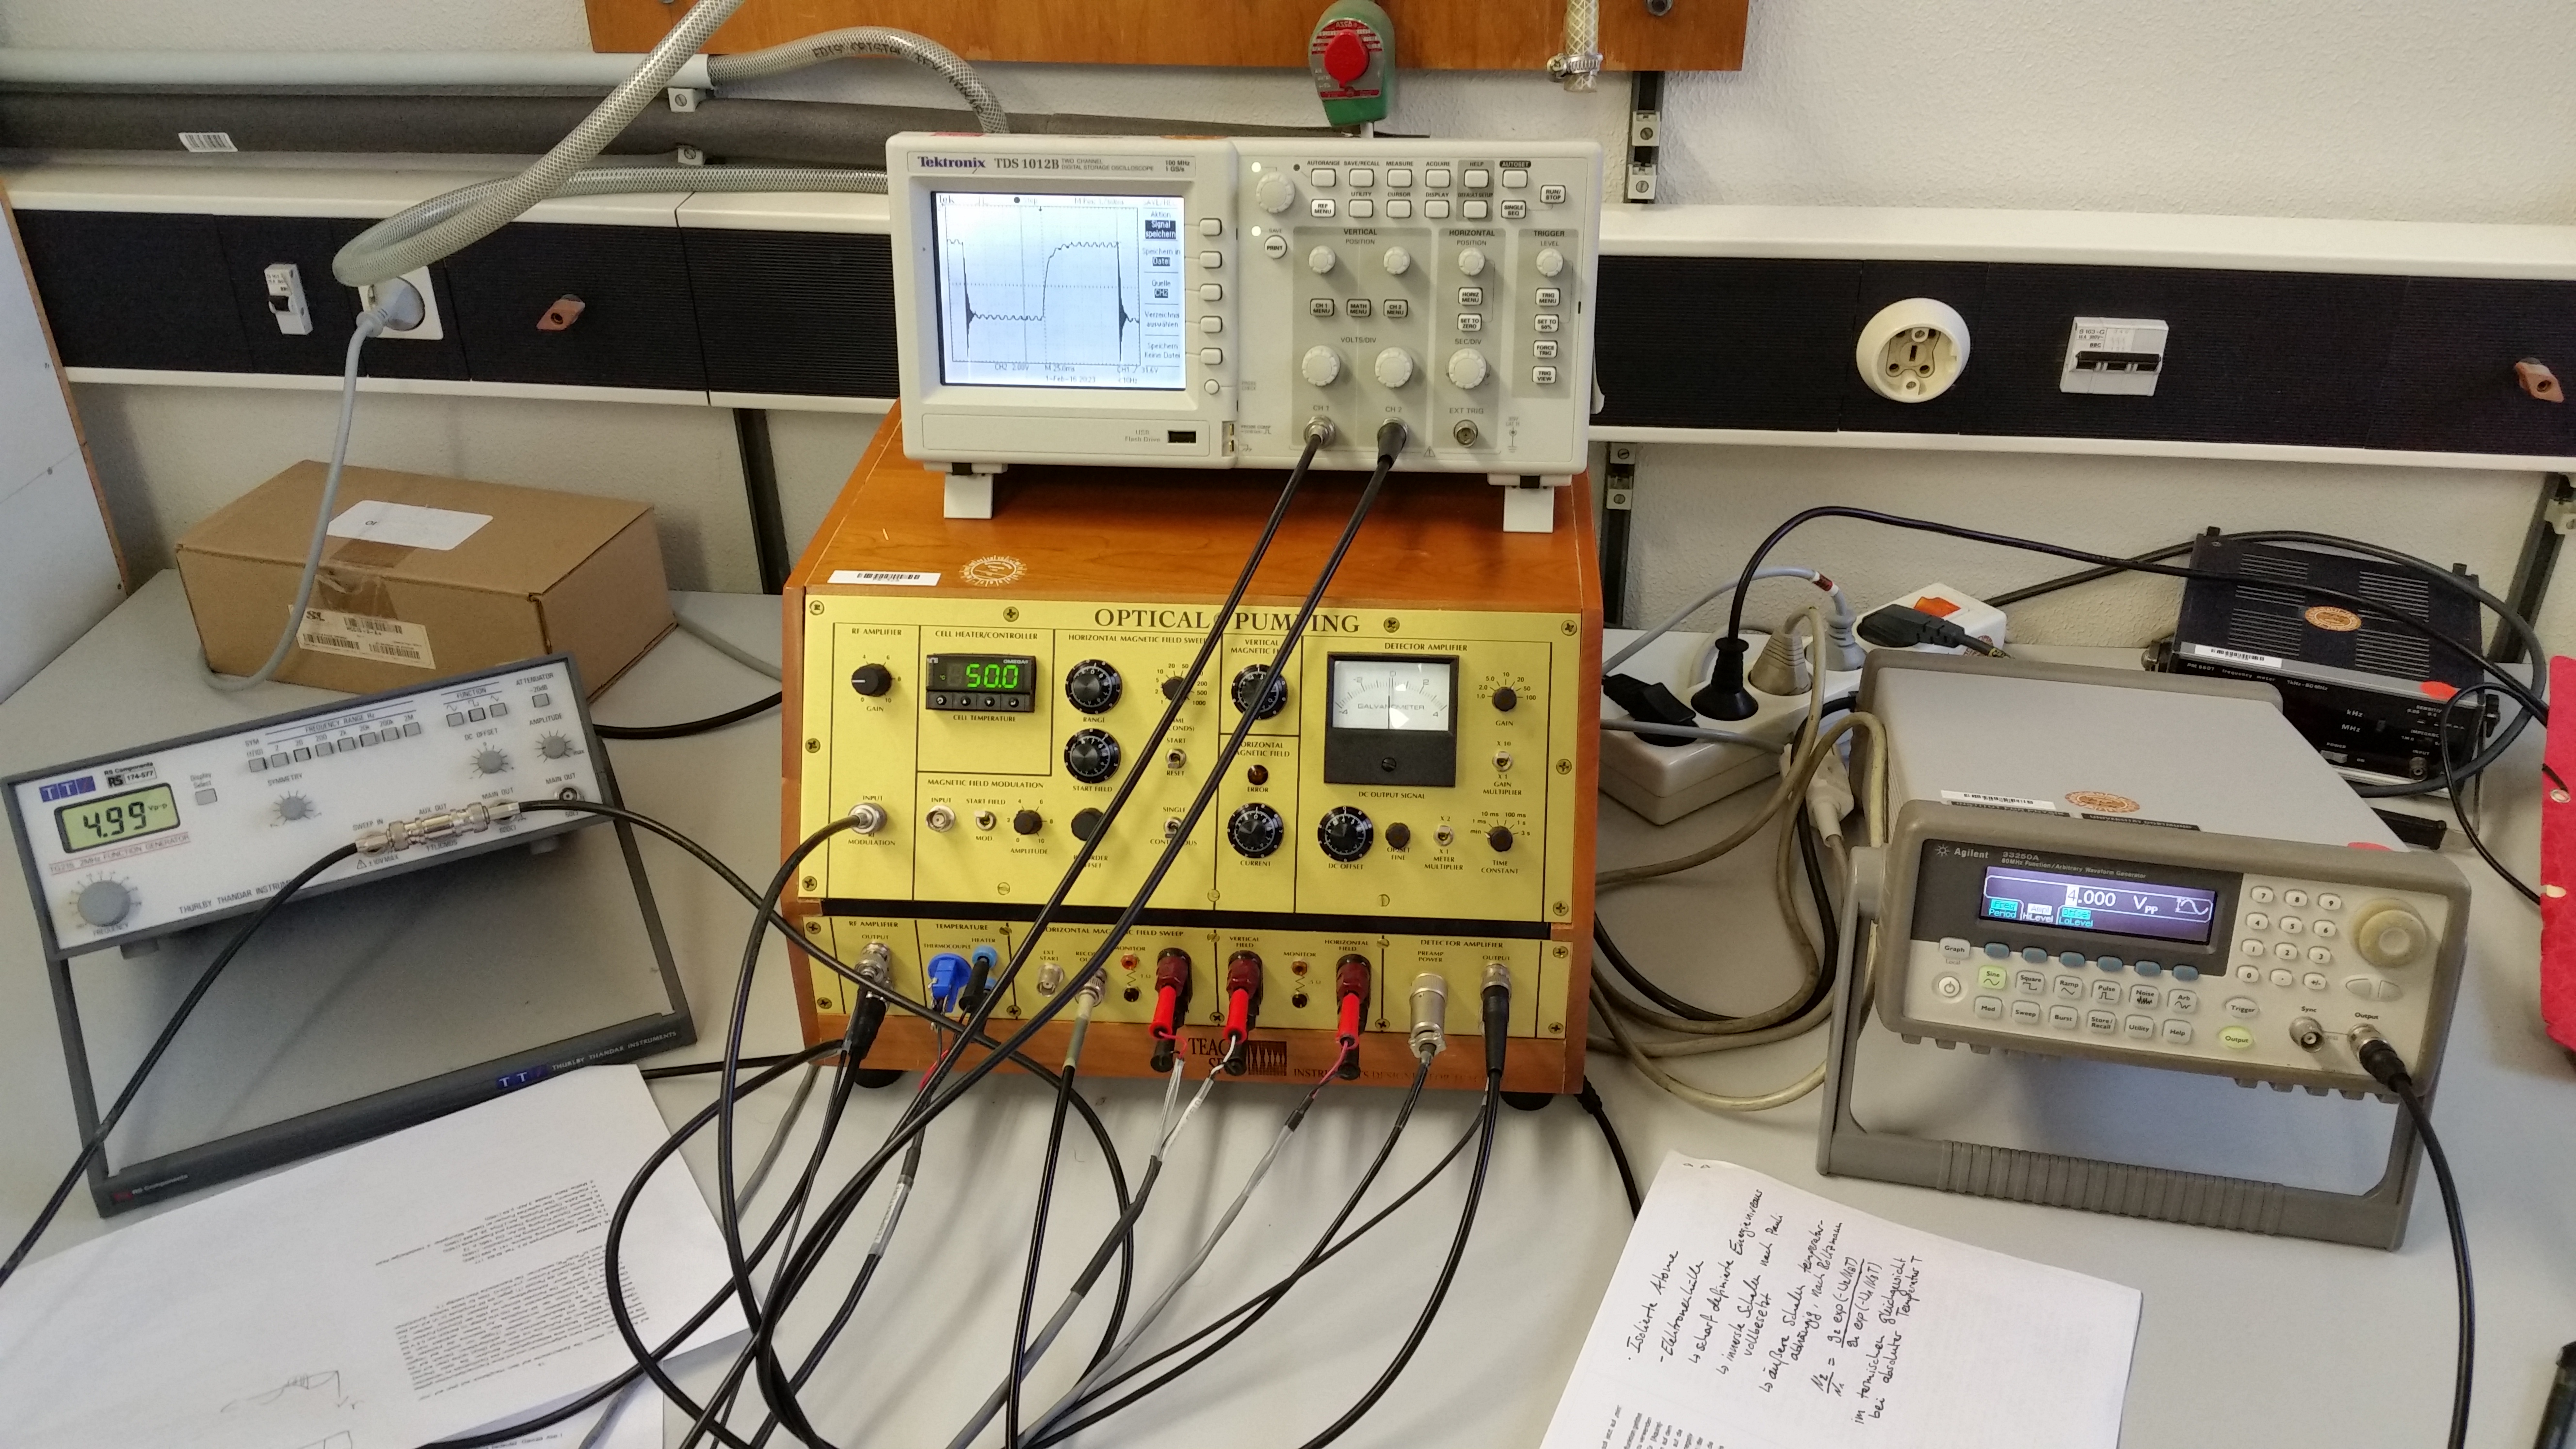
\includegraphics[trim = 0mm 200mm 50mm 100mm , clip ,width = \textwidth]{../Grafiken/Aufbau_Controlltafel.jpg}};
				
				%\draw[black](5,5.5) -- (6,5.5);
				\fill[gray!60!white](5.7,6.4) circle (0.4);
				\draw(5.7,6.4) circle (0.4);
				\node at (5.7,6.4) {$\boldsymbol 6$};
				
				\fill[gray!60!white](5.2,4) circle (0.4);
				\draw(5.2,4) circle (0.4);
				\node at (5.2,4) {$\boldsymbol 7$};
			
				\fill[gray!60!white](15,2.5) circle (0.4);
				\draw(15,2.5) circle (0.4);
				\node at (15,2.5) {$\boldsymbol 8$};
				
				\fill[gray!60!white](0.7,3) circle (0.4);
				\draw(0.7,3) circle (0.4);
				\node at (0.7,3) {$\boldsymbol 9$};
				
				%\draw(11,3) -- (9.8,3.2);
				%\draw(11,3) -- (9.7,2.8);
				%\draw(11,3) -- (9.3,2.3);
				%\fill[gray!60!white](11,3) circle (0.4);
				%\draw(11,3) circle (0.4);
				%\node at (11,3) {$\boldsymbol 7.1$};
				
				%\draw(11,1.8) -- (9.61,2.3);
				%\fill[gray!60!white](11,1.8) circle (0.4);
				%\draw(11,1.8) circle (0.4);
				%\node at (11,1.8) {$\boldsymbol 7.2$};
				
				%\fill[gray!60!white](5.2,4) circle (0.4);
				%\draw(5.2,4) circle (0.4);
				%\node at (5.2,4) {$\boldsymbol 7$};
			\end{tikzpicture}
			\caption{Oben: Der Verwendete Versuchsaufbau der optischen Pumpe.\\ Unten: Das Kontrollgerät mit dem die optische Pumpe gesteuert wird, die nötigen Generatoren, sowie das Oszilloskop für die auslese.}
			\label{fig:Versuchsaufbau}

\end{figure}

In \cref{fig:Versuchsaufbau} ist der verwendete Versuchsaufbau dargestellt.
Das Licht für die Anregung kommt von einer Spektrallampe (1), das Licht wird mithilfe einer Sammellinse (2.1) gebündelt und danach mithilfe eines $D_1$-Filters (2.2) auf die Nötige Anregungswellenlänge gefiltert. 
Danach wird mit einem Linearpolarisator (2.3) und einer $\lambda/4$-Platte (2.4) zirkular-polarisiertes Licht welches auf die Dampfzelle (4) fällt. Nach der Dampfzelle steht eine Sammellinse (2.5) die das Licht in eine Photodiode (5) Fokussiert, die Diode ist an einem Oszilloskop (6) angeschlossen.\\
Im Aufbau befinden sich zwei Helmholz-Spulenpaare , eine Vertikale (3.1) und eine Horizontale (3.2), dabei ist über die Horizontale Helmhotz-Spule eine Sweep-Spule gewickelt.
Die Spulen können über das Kontrollgerät (7) einzeln eingestellt werden.\\
Weiter wird ein Hochfrequenzgenerator (8) zum betrieb der Spule benötigt und ein Generator (9) für niedrigere Frequenzen um eine Modulation des Magnetfeldes zu erzeugen.\\
Die Heizung der Dampfzelle wird eine halbe Stunde bevor der Messung angestellt, um einen optimalen Dampfdruck zu erzeugen.
Der fertige Versuchsaufbau muss abgedunkelt werden.\\
\subsection{Messprogramm}
\subsubsection{Kompensation des Erdmagnetfeldes}
Zunächst muss der Aufbau so gedreht werden das er parallel beziehungsweise antiparallel zu der Horizontalkomponente des Erdmagnetfelds steht. 
Als nächstes wird die Vertikalkomponente ausgeglichen.
Dazu wird zunächst die Diode auf Kanal 2 des Oszilloskops gegeben und auf Kanal 1 wird der Recorder-Ausgang der Sweepspule gelegt und das Oszilloskop wird auf XY Betrieb gestellt.
Auf dem Oszilloskop sollte ein breiter nach unten gerichteter Peak zusehen sein, dieser wird mithilfe der Vertikalspule auf minimale Breite gebracht.
\subsection{Messung der Resonanzstellen}
In dieser Messung wird von \SI{100}{\kilo\hertz} bis \SI{1}{\mega\hertz} , in \SI{100}{\kilo\hertz} schritten durch geführt.
Dabei wird für jeden schritt der Strom gemessen an dem die Resonanzstelle des Magnetfeldes liegt, ein mal für das Magnetfeld bei $B=0$ und für die beiden Isotope.
Die Sweep-Spule wird mithilfe des Schalters Start/Reset auf Reset gestellt, wodurch ein konstantes Magnetfeld in der Apparatur vorliegt.
Dabei ist der Strom der angelegt wird Proportional zu den Umdrehungen an dem Potentiometer.
Ab einer Frequenz von 200-300 \SI{}{\kilo\hertz}, muss mithilfe der zusätzlichen Horizontalenspule der Sweep-Bereich auf die Resonanzstelle erweitert werden.
\newpage
\subsection{Relaxation zur Bestimmung des Mischungsverhältnisses}
\begin{figure}[h!]
	\centering
	\includegraphics[angle = 90 , clip , trim = 50mm 50mm 30mm 70mm, width =  0.49\textwidth , height = 0.3\textwidth]{../Grafiken/Resonanz_1_Exp_Anstieg_05V.jpg}	\includegraphics[angle = 90 , clip , trim = 45mm 40mm 30mm 30mm , width = 0.49\textwidth , height = 0.3\textwidth]{../Grafiken/Resonanz_1_Relaxation_4V.jpg}
	\caption{Links: der Fall wo sich das Magnetfeld aufbaut.\\ Rechts: Der Relaxationsfall.} \label{fig:Relaxation}
\end{figure}
An den Input RF Modulation-Anschluss des Kontrollgeräts wird der zweite Generator angeschlossen.
Dieser wird mit einer Rechteckspannung, auf \SI{5}{\hertz} und 0-5\si{\volt} eingestellt.
Die Rechteckspannung sorgt dafür das im Wechsel ein Schwingfall beziehungsweise der Relaxationsfall vorliegt und ein Phase in der sich das Magnetfeld im System wieder aufbaut. Diese beiden Fälle sind in \cref{fig:Relaxation} dargestellt.
Der Generator wird weiter noch auf Kanal 1 des Oszilloskops gestellt.
Dieses wird auf den YT-betrieb umgestellt und der Trigger wird auf die positive Flanke von Kanal 1 gestellt.
Hier wird die Aufsteigende Flanke wie links in \cref{fig:Relaxation} dargestellt aufgenommen, mithilfe des Oszilloskops.
%Hier wird die Spannung des Hochfrequenzgenerators von 1-10\SI{}{\volt} in \SI{1}{\volt} schritten durchgegangen und die Daten vom Oszilloskop ausgelesen, wobei die Mittlungsfunktion des Oszilloskops verwendet wurde.
Der Trigger wird auf die negativen Flanke umgestellt.
Und es wird in den Relaxationsbereich der Nach der aufsteigenden Flanke ist hinein gezoomt, dieser ist Rechts in \cref{fig:Relaxation} dargestellt.
Dies wird für Spannungen von 1-\SI{10}{\volt} in \SI{1}{\volt} schritten wiederholt und ebenfalls für beide Isotope durchgeführt.
%Dies wird wiederholt, nur wird der Trigger auf die abfallende Flanke eingestellt und in den Relaxationsbereich hinein gesoomt.


\newpage
\subsection{Angaben zur Apparatur}
\begin{table}[h!]
	\centering
	\begin{tabular}{l c c c c}
	\toprule
	Spule & Radius & Windungszahl & Maximalstrom & Potentiometer\\
	& $R/\SI{}{\centi\meter}$ & $N$ & $I_\text{max}/\SI{}{\ampere}$ & Umdrehung/\SI{}{\ampere}\\\midrule
	Sweep-Spule & 16,39 & 11 & 1 & 0,1\\
	Horizontale-Spule & 15,79 & 154 & 3 & 0.3\\
	Vertikale-Spule & 11,735 & 20 & 1 & 0.1\\
	\bottomrule
	\end{tabular}
	\caption{Die angaben zu den Spulen die für die zur Bestimmung der des angelegten Magnetfeldes Relevant sind.\cite{V21}}\label{tab:Apparatur}
\end{table}
In \cref{tab:Apparatur} sind die Angaben zu den Einzelnen Spulen gegeben.
Um daraus das nötige herrschende Magnetfeld zu bestimmen wird die Formel für die Herlmholtz-Spule benötigt:
\begin{align}
	B=\mu_0\frac{8}{\sqrt{125}}\frac{N\cdot I}{R}
\end{align}